\section{Mathematical model for the description of the PMT's response}


We started by using a model for signal amplitude distribution based off of Gaussian single photoelectron spectra as discussed in \cite{Bellamy:1994bv} that works reasonably well for H8500, but this model does not satisfactorily treat the spectra seen in the new H12700 MAPMTs from Hamamatsu. Consequently, Pavel Degtyarenko~\cite{DEGTIARENKO20171} has developed a more complicated model using several Poisson components to better fit the MAPMT spectra, especially in the single photoelectron cases.
This mathematical model features a realistic descripription of the MAPMT response where each parameter corresponds to the physical process inside the MAPMT.
The SPE spectrum is fitted with a function used to describe the signal amplitude distribution measured by the MAPMT as shown on Fig.~\ref{fig:SPEfit},
The probability of an initial photon to knock out a photoelectron is distributed according to the Poissonian $P(m;\mu)=\frac{\mu^me^{-\mu}}{m!}$.
To approximate the performance of the first amplification cascade of the MAPMT the function $T(n,m;t)$ is introduced in the model as trinomial sum of three Poissonians with different average secondary multiplicities and the corresponding three relative probabilities for every photoelectron to generate secondary electrons.
The function $G(a,n;\sigma)$ corresponds to the realistic DAQ measurement function to introduce the experimental resolution into the resulting model function.

\begin{figure}[bt]
	\centering
	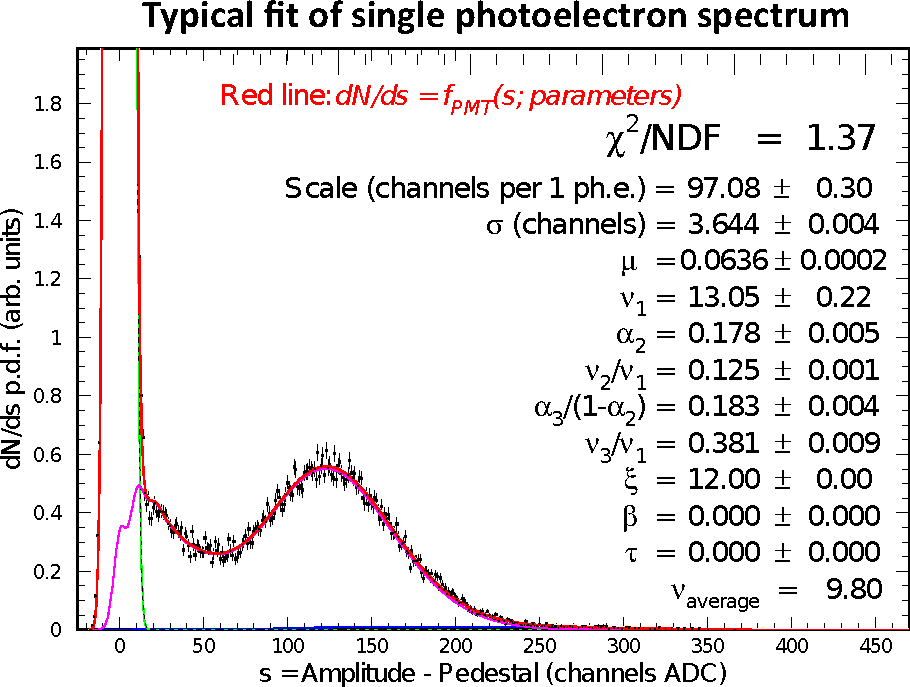
\includegraphics[width=\linewidth]{figures/SPEfit.pdf}
	\caption{Sample of single photoelectron spectrum from one of the pixels at 1000 V with low intensity laser light source,
where integer $m$ corresponds to the number of photoelectorns created at the first stage of the photodetector (photocathode) by the incident light during one event of radiation, index $n$ corresponds to the number of electrons generated at the second stage of the photodetector (first dynode).
}
\label{fig:SPEfit}
\end{figure}

The model is found to describe well the amplitude distributions measured at different levels of radiation with different supply voltages.
The parameters provide MAPMT characteristics independently of the test measurement conditions (see Fig.~\ref{fig:PavelPassport}): the $scale$ parameter is virtually independent on the light radiation level while strongly dependent on high voltage supply, the exact behavior one would expect from the characteristic of internal dynode system of MAPMT.

\begin{figure}[t]
	\centering
	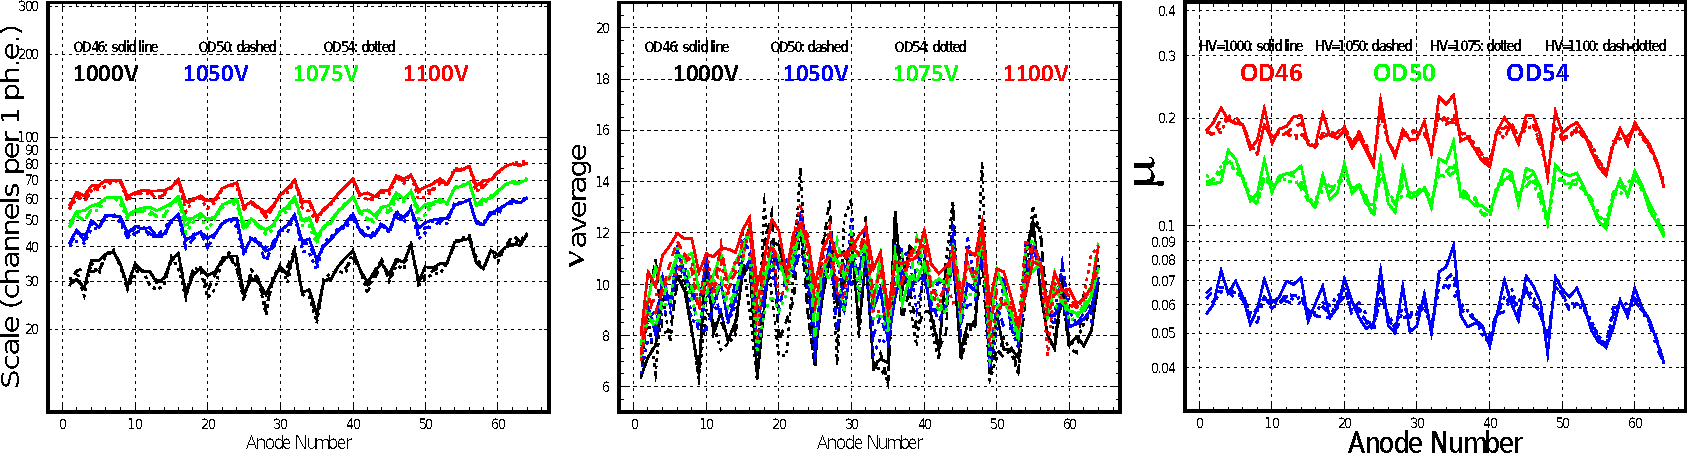
\includegraphics[width=\linewidth]{figures/PavelPassport.pdf}
	\caption{Distributions of fit parameters among the pixels for measurements with 4 different high voltage supplies and 3 different light intensities: the parameter $scale$ characterizes the amplification (dynode) system, $\nu$ - first dynode performance, $\mu$ relates to the quantum efficiency (photocathode performance).}
	\label{fig:PavelPassport}
\end{figure}

Currently we have tested 80 H8500 and 260 H12700 (the largest collection of these new MAPMTs in the world).
The accumulated data provide an immense knowledge about quantum and collection efficiencies of MAPMTs, their surface uniformity, single photoelectron (SPE) spectrum resolution etc.
This parameterized information extracted from the fit of each pixel for every MAPMT is used to describe the detector response in the future simulation.

